\documentclass[conference]{IEEEtran}
\IEEEoverridecommandlockouts
% The preceding line is only needed to identify funding in the first footnote. If that is unneeded, please comment it out.
\usepackage{cite}
\usepackage{amsmath,amssymb,amsfonts}
\usepackage{algorithmic}
\usepackage{graphicx}
\usepackage{textcomp}
\usepackage{longtable}
\usepackage{xcolor}
\def\BibTeX{{\rm B\kern-.05em{\sc i\kern-.025em b}\kern-.08em
    T\kern-.1667em\lower.7ex\hbox{E}\kern-.125emX}}
\begin{document}

\title{Explorando Retrieval-Augmented-Generation como solução para Memória Episódica\\
{\footnotesize \textsuperscript{*}Note: Trabalho desenvolvido para a Disciplina de T.E.I.: Generative Pre-Trained Transformers}
}

\author{\IEEEauthorblockN{1\textsuperscript{st} Antonio Lucio Braga Secchin}
\IEEEauthorblockA{\textit{Centro Tecnológico} \\
\textit{Universidade Federal do Espírito Santo}\\
Vitória, Brasil \\
antonio.secchin@edu.ufes.br}
\and
\IEEEauthorblockN{2\textsuperscript{nd} Bruno Lopes Altoé}
\IEEEauthorblockA{\textit{Centro Tecnológico} \\
\textit{Universidade Federal do Espírito Santo}\\
Vitória, Brasil \\
bruno.altoe@edu.ufes.br}
\and
\IEEEauthorblockN{3\textsuperscript{rd} Rhuan Garcia de Assis Teixeira}
\IEEEauthorblockA{\textit{Centro Tecnológico} \\
\textit{Universidade Federal do Espírito Santo}\\
Vitória, Brasil \\
rhuan.teixeira@edu.ufes.br}
}

\maketitle

\begin{abstract}
Esse documento relata a implementação experimental de um assistente virtual, utilizando-se das técnicas de RAG e embeddings para simular a memória episódica. É descrita a metodologia utilizada para o desenvolvimento da aplicação, como também avaliado seus resultados na seção de experimentos. No geral, o modelo apresentou desempenho positivo em conversas simples e recuperação de memória básica, além de conseguir guardar novas memórias. Porém, em tarefas mais complexas dependente dos contextos, apresenta dificuldades. Possíveis melhoras podem incluir fine-tuning do modelo, além do uso de estruturas mais simples como BERT para classificação de relevância de uma conversa.
\end{abstract}

\begin{IEEEkeywords}
RAG, Large-Language-Models, Episodic memory, Retrieval-Augmented-Generation
\end{IEEEkeywords}

\section{Introdução}
A memória episódica, enquanto conceito inspirado nos processos cognitivos humanos, vem ganhando destaque no campo dos modelos de linguagem de larga escala (LLMs). A incorporação de mecanismos de memória episódica permite que os sistemas armazenem e recuperem experiências específicas, proporcionando respostas mais contextualizadas e personalizadas, junto com um conjunto novo de funcionalidades. Este atigo explora essa idéia, demonstrando como, utilizando do modelo DeepSeek R1 e um sistema de Retrieval Augmented Generation construído em python com uso de ChromaDB para armazenar e buscar embeddings similares, é possivel simular aspectos de uma memória episódica. Ao utilizar de vetores para armazenar as memórias, Retrieval-augmented generation para filtrar elas e organizar as mais relevantes, usando-as como entrada para um modelo de linguagem de larga escala, conseguimos simular a existência de uma memória para nossa inteligência artificial.
O artigo está estruturado pelas seguintes sessões: resumo, introdução, trabalhos correlatos, metodologia, experimentos, resultados e bibliografia. A seguir, trabalhos correlatos indicará as principais fontes de conhecimento relacionadas com a implementação de RAGs em inteligências artificiais. Metodologia, por sua vez, explicará as estratégias que serão utilizadas nos experimentos em mais detalhes, como o uso de embeddings para armazenamento da base de dados e criação de memórias formatadas em Json. Experimentos demonstrará essas estratégias de fato sendo utilizadas para a criação de um assistente virtual com memória episódica, e resultados explicitará as capacidades finais desta implementação.

\section{Trabalhos correlatos,}

\subsection{Episodic Memories Generation and Evaluation Benchmark for Large Language Models}
O paper propõe um benchmark abrangente para avaliar a capacidade de memória episódica em Modelos de Linguagem de Grande Escala (LLMs), nele se destaca que LLMs atuais, apresentam dificuldades significativas ao lidar com tarefas que envolvem múltiplos eventos relacionados ou relacionamentos espaço-temporais.

O benchmark é estruturado para avaliar LLMs em diversas tarefas de memória episódica, abrangendo desde a capacidade de recuperar eventos específicos até o rastreamento de estados de entidades/personagens e ordenação cronológica de eventos. Para isso, o trabalho introduz um framework que gera narrativas sintéticas com dados controlados sobre eventos e contextos, permitindo avaliar a performance dos modelos em tarefas de recuperação de memória episódica.
É valido notar que esses eventos, similares as nossas memórias desse paper, sempre contém algo similar a um cabeçalho contendo data, local, entidades e o conteúdo do evento.

\section{Metodologia}
Para simular uma memória episódica utilizamos de embeddings de memórias, que serão melhor explicadas a seguir, para salvar tais informações de forma fácil de se recuperar para o nosso modelo, entretanto, não é uma boa estratégia apenas inserir toda a conversa entre o agente e o usuário como uma memória, já que as informações seriam brutas e conteriam bastante conteúdo desnecessário. Logo, com esses objetivos pensamos em utilizar um arquivo, uma string seguindo formato Json para cada memória, contendo alguns campos importantes. Dois que merecem destaque são: \textbf{Session} que tenta resumir a situação em uma ou duas palavras chaves, como por exemplo: "Almoço", "Ao acordar"; e o campo \textbf{Description} que como seu nome indica relata o acontecimento em si, contendo normalmente o que é buscado pelo usuário e retornado pelo modelo. Um exemplo dos dados que são armazenados em um Json seguindo nosso formato pode ser visto na tabela \ref{tab:Json}. 

\begin{table}[h]
    \centering
    \begin{tabular}{c|c}
    \textbf{Campo} & \textbf{Valor} \\ 
    \hline
    \textbf{Date} & 2025-02-26 \\ 
    \hline
    \textbf{Time} & 07:35:00 \\ 
    \hline
    \textbf{Period} & Manhã \\ 
    \hline
    \textbf{Day\_of\_week} & Terça-feira \\ 
    \hline
    \textbf{Season} & Verão \\ 
    \hline
    \textbf{Session} & Ao acordar \\ 
    \hline
    \textbf{Description} & Descrição do evento
    \end{tabular}
    \caption{Exemplo de Json (memória)}
    \label{tab:Json}
\end{table}

Mesmo que as informações tenham sido reduzidas, com o passar do tempo sua quantidade pode ser exorbitante e inviável de se colocar no prompt por completo. Para contornar tal situação adotamos a utilização de uma estrutura de Retrieval-Augmented Generation que analisa a base de dados transformada em embenddings e retorna as 3 memórias mais prováveis de serem relacionados a pergunta do usuário. Para alcançar esse objetivo utilizamos do modelo "granite-embedding" para gerar os embeddings e ChromaDB para armazenar os vetores e textos relacionados, além de recuperar os embeddings mais próximos da pergunta. 
Após adquirir as memórias julgadas mais significantes, essas são inseridos em uma prompt contendo a pergunta, mensagem, do usuário, para que o LLM escolhido DeepSeek-R1 consiga analisar os dados e responder o usuário com base no contexto provido de situações passadas presentes nas infromações guardadas.

\subsection{Criação e Busca de memórias}
Para filtrar os conteúdos e criar novas memórias Json foi utilizado do DeepSeek-R1, recebendo como argumento o histórico da conversa, contendo as entradas do usuário e respostas do assistente. Ele foi encarregado de classificar como uma informação relevante ou não a ser armazenada e resumir o conteúdo no Json resultante. Para auxiliar no processo, informações temporais como data, horário, estação foram decididas previamente pelo código, usando como base o momento de envio da mensagem do usuário. No fim se a informação for julgada relevante, ela é inserida na base de dados.

De forma semelhante a forma utilizada para criar novas memórias, para buscar as memórias mais semelhantes e relacionadas a pergunta do usuário, foi utilizado o DeepSeek-R1 para gerar uma memória sobre aquela pergunta, estimando com base na pergunta e tempo atual uma data, tempo, período, session e description para essa memória criada, essa memória então passa pelo modelo de embedding e é buscada no ChromaDB para retornas as memórias mais relacionadas e ser inserida como contexto para a pergunta do usuário.

Para simplificar o entendimento, podemos ver o sistema de forma mais simples na figura\ref{fig:Estrutura} que demonstra como a informação do usuário trafega no sistema. 

\begin{figure}[h]
    \centering
    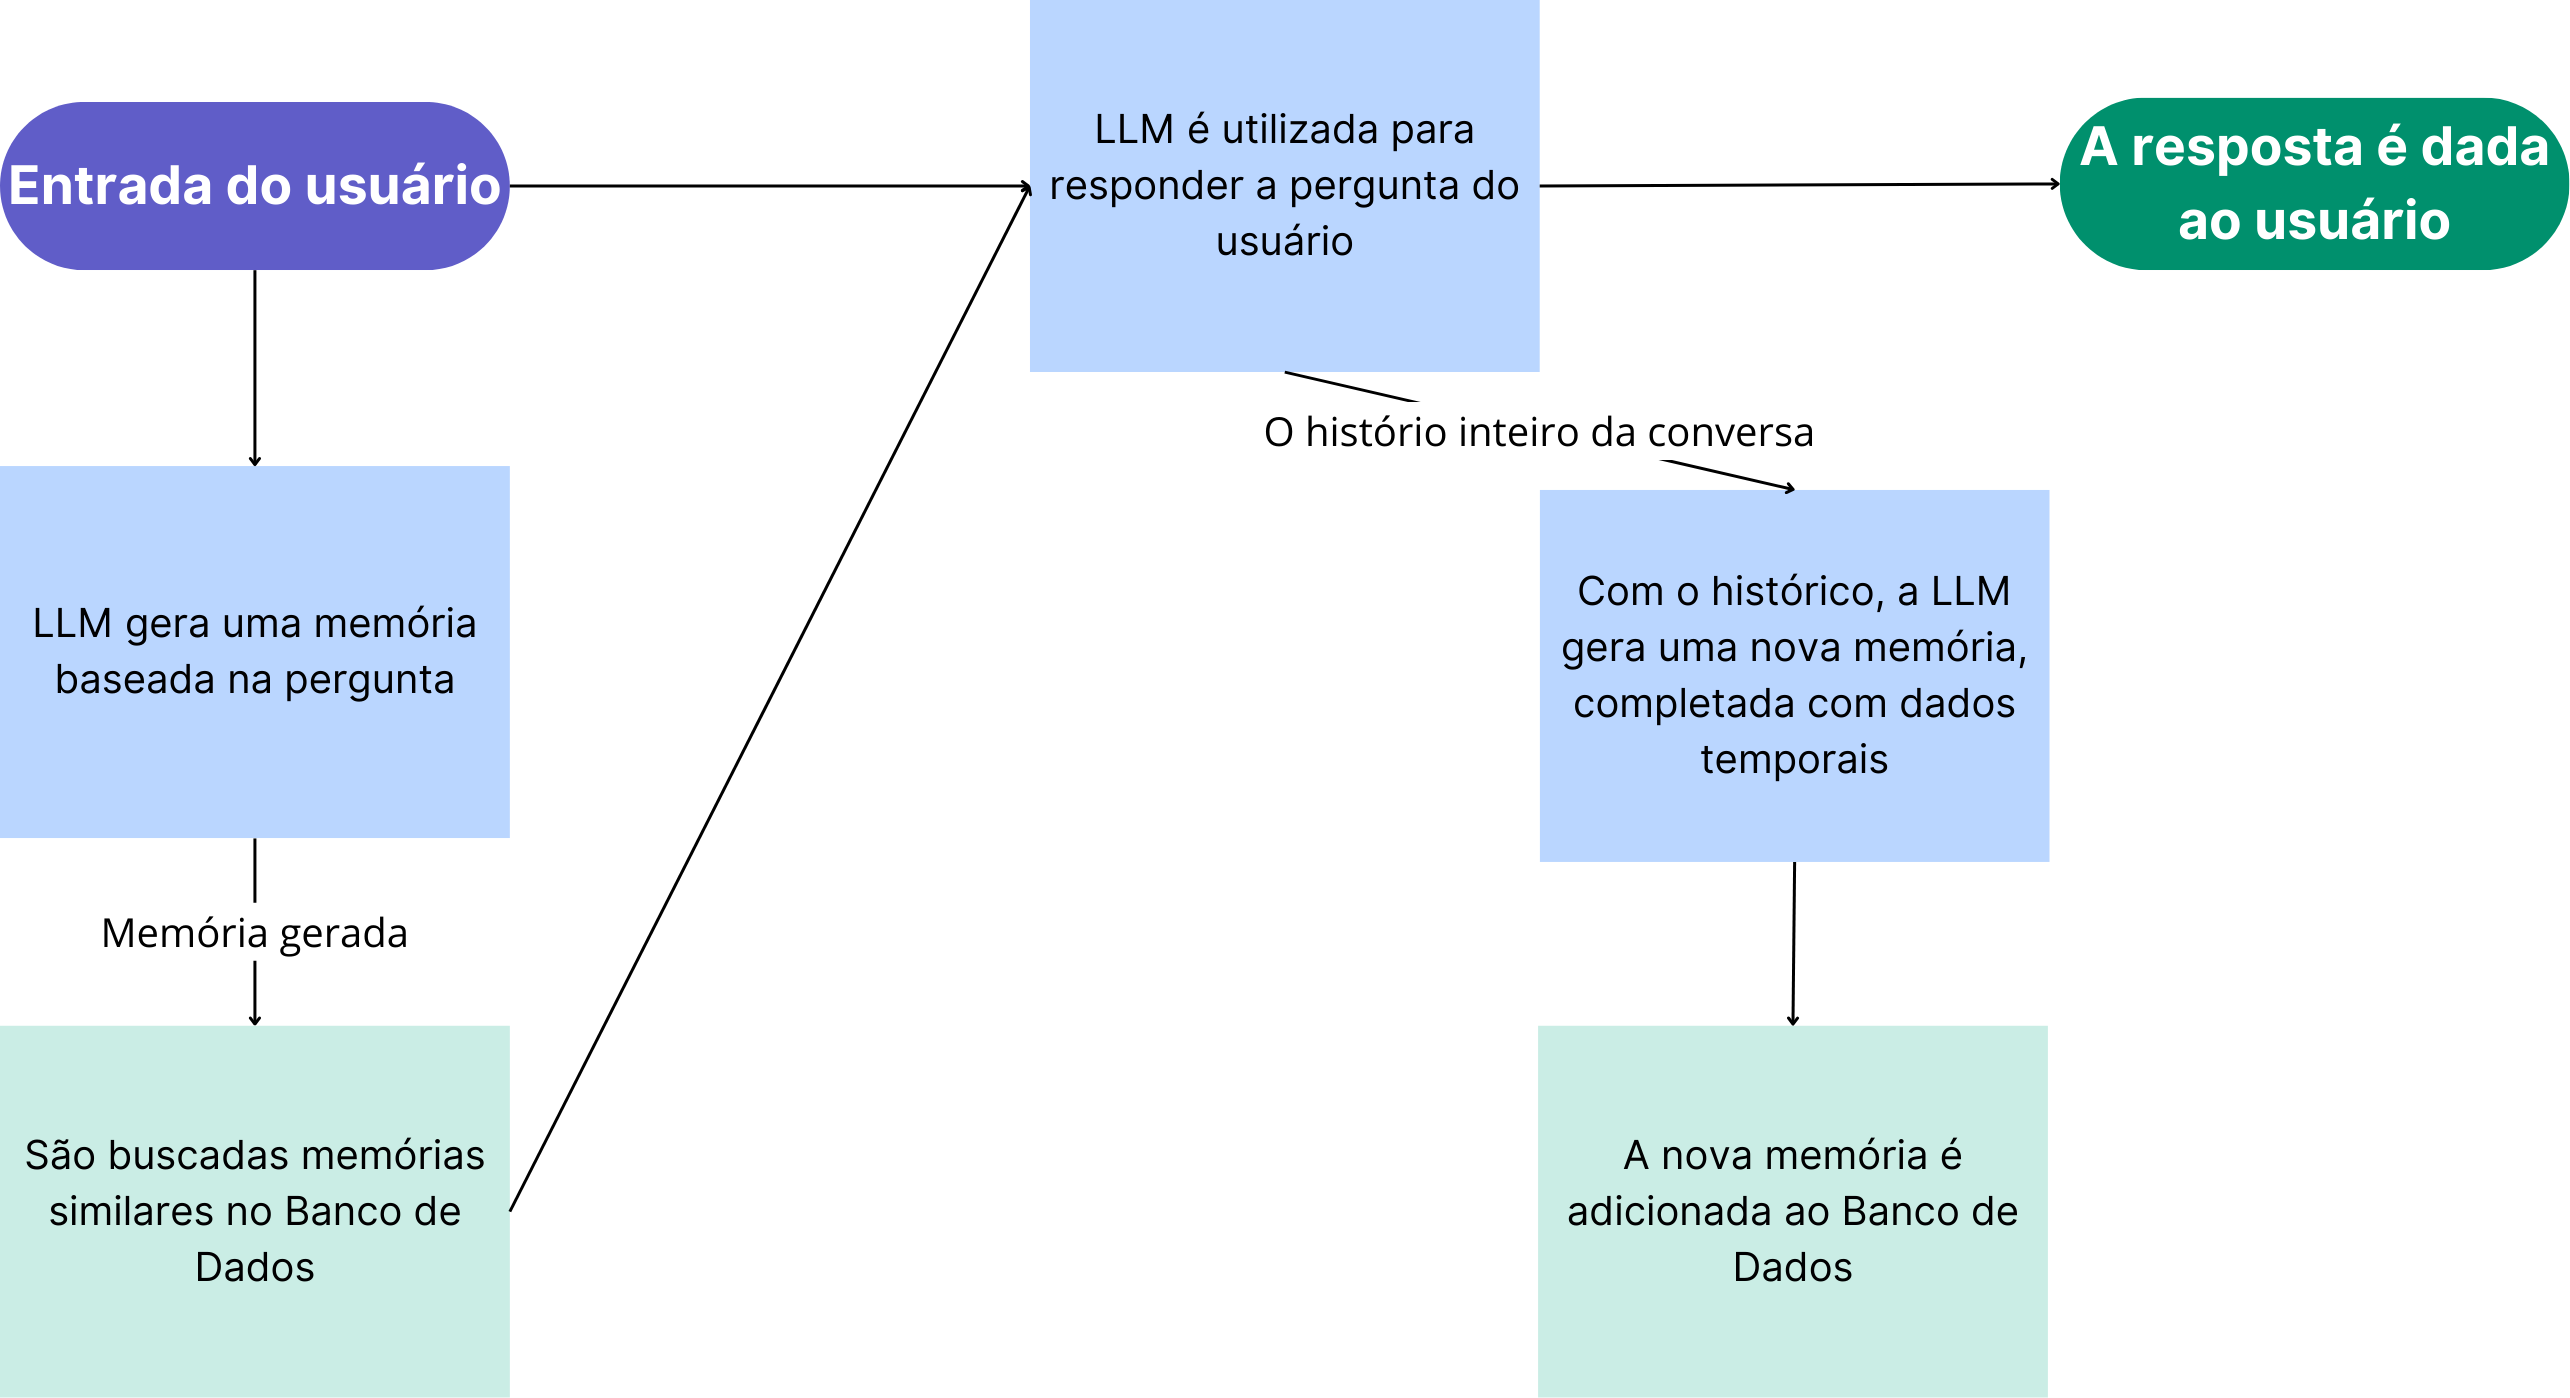
\includegraphics[width=0.5\linewidth]{Estrutura do sistema.png}
    \caption{Fluxo dentro do sistema construído}
    \label{fig:Estrutura}
\end{figure}

\subsection{Ambiente}
Em busca de ter uma interface mais agradável foi utilizado a biblioteca Gradio para auxiliar na criação de uma página web e uma interface de chatbot. Ela também proporcionou a conveniência de retornar o histórico de conversa em um formato de fácil manipulação, facilitando a implementação do código.

Para facilitar o desenvolvimento e testes, foi formulada uma base de memórias iniciais do sistema seguindo o padrão já descrito e exemplificado na tabela 1. Assim pudemos ajustar os prompts para melhor lidar com o formato escolhido e testar todas funcionalidades do sistema.

\subsection{Embedding}
Com base nas experiências iniciais durante o desenvolvimento e graças a essa base, identificamos um problema com a forma em que o modelo de embedding escolhido lidava com o formato escolhido para armazenar nossas memórias, a diferença de importância dada aos campos era grande e os campos como data, horário e período tinham pouco impacto no embedding final devido a quantidade pequena de tokens quando comparados ao campo de descrição. Para lidar com isso enquanto limitados por não ter capacidade de criar um modelo de embedding novo específico ao problema, pensamos na solução de calcular o embedding dos campos menores em tamanho separados do conjunto e então somar o embedding dos campos menores ao embedding tradicional obtido sob a memória inteira, utilizando também de multiplicadores para melhor lidar com os "pesos", com isso obtivemos assim resultados mais consistentes ao fazer o retrieval a partir da query e tornou mais confiável a expectativa de que as memórias resgatadas serão relevantes.

\section{Experimentos}

Os testes foram realizados por meio do uso da interface criada pelo gradio. Sua função retorna uma mensagem em formato de string, e uma lista de dicionários representando a conversa até aquele ponto (chamado de \textit{"history"}). A resposta do agente é visível pela interface gráfica facilitando sua avaliação.

Primeiramente, foram feitos testes com perguntas sobre memórias já inseridas previamente na base de dados (memórias presentes em nosso dataset) com o objetivo de analisar o comportamento do assistente com os resultados devolvidos pela RAG, a capacidade de conferir os elementos mais próximos escolhidos e retornar o acontecimento requisitado com boa qualidade do texto. O exemplo da figura \ref{fig:primeiro_exemplo} demonstra um teste realizado pedindo para retornar a ida a um restaurante italiano no dia 26/02.

Outro tipo de teste realizado, foi a inserção de dados pela interface gráfica que é escolhida ser inserida ou não de acordo com o julgamento do modelo. A partir do momento da inserção de uma nova informação, foi realizado dois testes. O primeiro é a recuperação da informação durante a mesma seção (vide imagem \ref{fig:add_mem}), utilizando tanto o histórico da conversa quanto o contexto fornecido de outras memórias. Outro caso é entre seções diferentes, analisar se o assistente é capaz de retornar a informação utilizando apenas das informações adquiridas pela RAG. 

\begin{figure}[h]
    \centering
    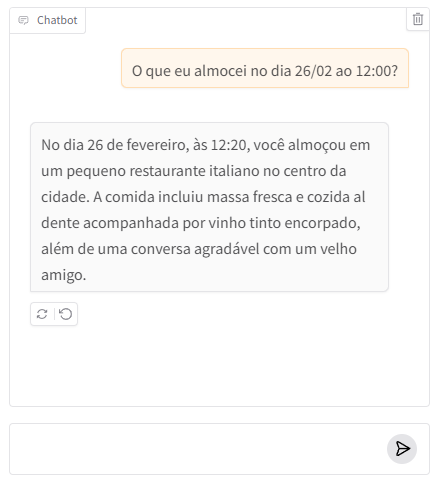
\includegraphics[width=0.5\linewidth]{primeiro_exemplo.png}
    \caption{Resposta do assistente utilizando a base de dados}
    \label{fig:primeiro_exemplo}
\end{figure}

\begin{figure}[h]
    \centering
    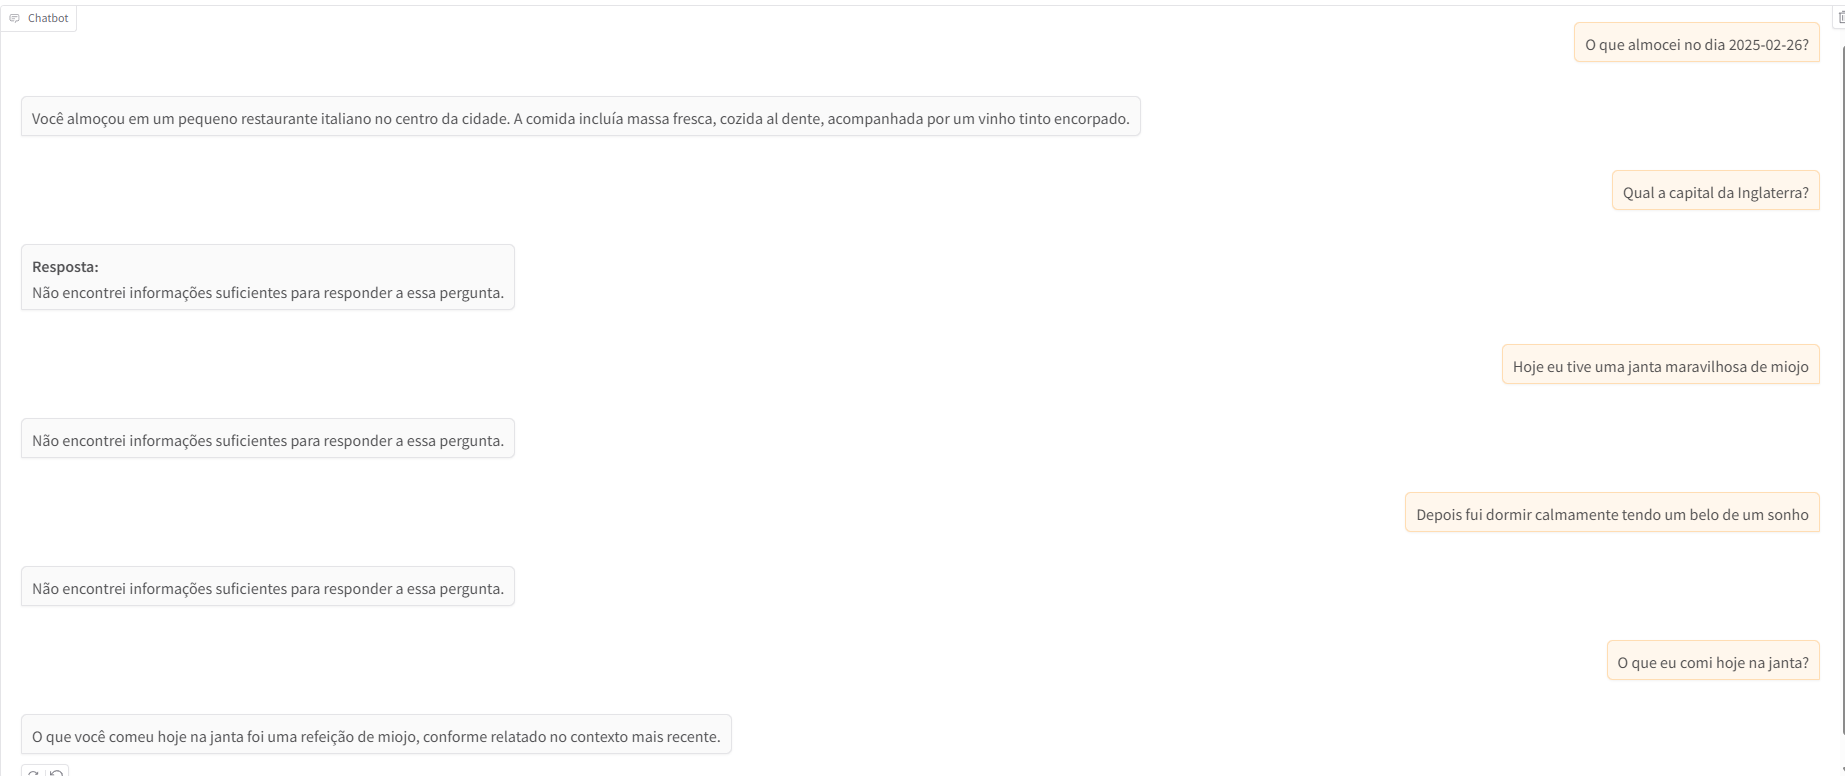
\includegraphics[width=1\linewidth]{terceiro_exemplo.png}
    \caption{Adição de memória e conversa contínua}
    \label{fig:add_mem}
\end{figure}


\section{Resultados}

A combinação de uma RAG junto com uma LLM, trouxeram resultados positivos, demonstrando uma capacidade de recapitular eventos salvos na base de dados, analisando os resultados da RAG e capturando o correto. Foram realizados testes requisitando dados salvos na mesma seção da qual foram armazenados e em outra seção, em ambas as situações o assistente conseguiu retornar o contexto requisitado.
Uma dificuldade encontrada no processo de armazenar conversas, foi descobrir maneiras para que a inteligência artificial marque a iteração como relevante, esse resultado pode ser fruto de não utilizarmos os melhores modelos por limitações técnicas.

A capacidade do agente como chatbot geral foi levemente afetada ao utilizar o prompt preparada, e perguntas simples como "Me diga um pouco sobre o Brasil" podem retornar resultados inesperados influenciados pelas memórias inseridas que contenham palavras em comum por exemplo, isso pode ser visto na figura \ref{fig:Brasill}. 
\begin{figure}[h]
    \centering
    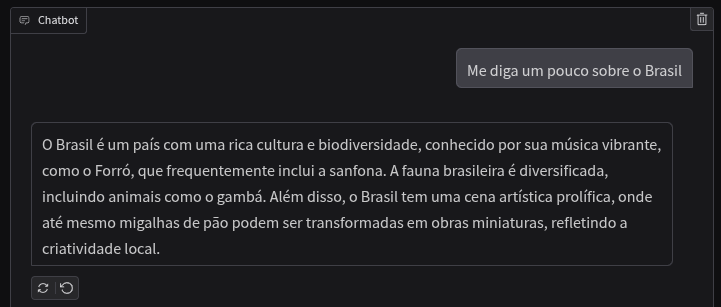
\includegraphics[width=0.5\linewidth]{Conte sobre o brasil.png}
    \caption{Exemplo - Conte sobre o Brasil}
    \label{fig:Brasill}
\end{figure}

Também foram observados momentos em que o modelo misturou algumas memórias do mesmo contexto e dia, algo que nem sempre resulta em boas respostas, um exemplo é o da figura \ref{fig:MisturaMem} em que foram misturadas as memórias de que foi encontrado um easter-egg na série de ficção científica (algo que aconteceu, pelos relatos, no horário da noite) com a memória de que ele ganhou um ingresso para um show de jazz (outra coisa que aconteceu, mas no horário da tarde).
\begin{figure}[h]
    \centering
    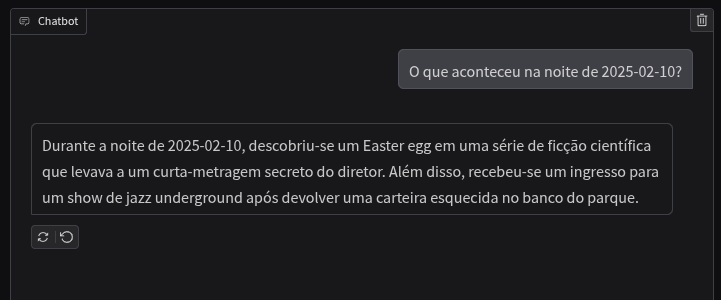
\includegraphics[width=0.5\linewidth]{Exemplo completo demais.png}
    \caption{Exemplo de memórias misturadas}
    \label{fig:MisturaMem}
\end{figure}


É valido destacar que o nosso sistema, mesmo em situações ideais, não irá conseguir lidar com tarefas mais complexas que envolvam mais de 3 memórias pela estrutura que escolhemos utilizar. Isso porquê mesmo que aumentássemos o número de memórias recapituladas pela query, o modelo passa a muitas vezes alucinar e não dar boas respostas mesmo com memórias boas de contexto. Algo compatível com o que podemos ver no artigo \cite{b1}

Porém de forma geral, foi observado (vide figura \ref{fig:ResulPos}) que o sistema se comporta bem para recapitular memórias simples e gerar novas em cima de uma conversa.
\begin{figure}[h]
    \centering
    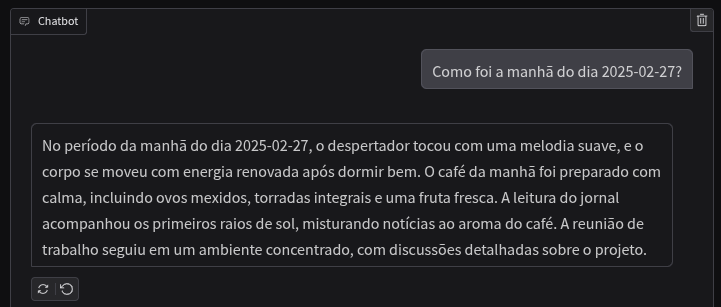
\includegraphics[width=0.5\linewidth]{ResultadoPositivo.png}
    \caption{Resultado Positivo}
    \label{fig:ResulPos}
\end{figure}




\section*{Trabalhos Futuros}

Após o desenvolvimento do sistema e execução dos experimentos, surgiram alguns temas que julgamos válidos de serem explorados no futuro. São eles: O desenvolvimento de um modelo de embedding modelado com um formato de memória, no nosso caso JSON, como foco principal, algo especializado que não precise de adaptações como a que foi feita por nós para obter um bom desempenho; E o fine-tuning do modelo de LLM usado na geração de memórias para que sigam uma estrutura mais consistente, sem problemas com JSONs mal formulados, o que facilitaria a conversão da resposta para JSON e provavelmente faria o sistema mais confiável. Outra possibilidade de melhoria, seria na classificação de quais memórias são relevantes a serem inseridas na base de conhecimento, imaginamos sobre a possibilidade de um modelo BERT com uma camada de saída específica para isso, mas não tivemos tempo de explorar esse caminho. 

\begin{thebibliography}{00}
\bibitem{b1}A. Huet, Z. Ben Houidi, and D. Rossi, “Episodic Memories Generation and Evaluation Benchmark for Large Language Models,” arXiv:2501.13121 [cs.CL], 2025. [Online]. Available: https://arxiv.org/abs/2501.13121

\end{thebibliography}

\end{document}
